\chapter{Analysis}\label{sec:analysis}
Sections~\ref{sec:analysis:examples:single} and~\ref{sec:analysis:examples:multiple} abstract and deduce the essential characteristics of any interaction.
These characteristics are relevant for a formalized language of \cmvs{}.
To accomplish this goal, the approach is to deduce the characteristics by a list of examples.
What are the expected data structures for each visualization?
What visual variables can be used to show an interaction?
A list of possible interactions is given for each visualization.
Those interactions will be classified according to \textcite{Yi2007} and the relevant subject of the interaction is specified.

Section~\ref{sec:analysis:requirements} gives a set of requirements which can be used to evaluate a framework of \cmvs{}.

Finally in Section~\ref{sec:analysis:frontend-framework-comparison} existing tools are evaluated with respect to their suitability for \cmvs{}.
In order to accomplish that, advantages and disadvantages of libraries and frameworks are compared and a final decision is made.

\section{Single Visualization Interactions}\label{sec:analysis:examples:single}

The data visualization catalogue by Severino Ribecca list many of the most used data visualizations\cite{VisualizationCatalogue2017}.
This section covers a list of common data visualizations from that catalogue as examples.
The expected data structure and a list of possible interactions is systematically analysed.

\textbf{Line graphs}
\begin{figure}
  \begin{center}
    \subfloat[Line graphs]{{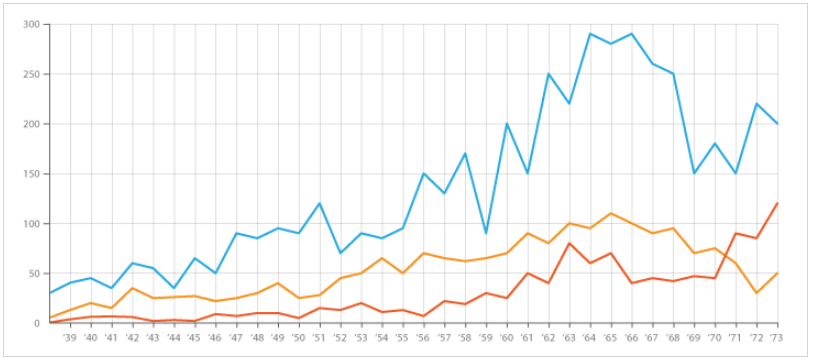
\includegraphics[width=0.4\textwidth]{figures/analysis/line-graphs} }}%
    \qquad
  \end{center}
  \caption{Line graphs are used to display trends}
  \label{fig:analysis:line-graphs}
\end{figure}

Line graphs display how quantitative values have changed over time.
They are perfectly suited to show trends or compare multiple series of data with each other.
The expected data format is \emph{tabular}, since one ore many series of data in parallel are visualized.

Line graphs are drawn in a Cartesian coordinate system, connecting subsequent points to each other.
Thus,
\begin{enumerate*}[label=(\arabic*)]
    \item position
    \item orientation and
    \item texture
\end{enumerate*}
are constrained by the nature of the visualization.
However, an interaction with the line graph can alter the
\begin{enumerate*}[label=(\arabic*)]
    \item shape
    \item color or
    \item size
\end{enumerate*}
of lines to create a visual effect.
It is further possible to highlight either the entire series of data or a single data point within that series, e.g. changing the shape and size of the point.
Table~\ref{tab:analysis:line-graph:interactions} shows a list of conceivable interactions in a line graph.

\begin{table}[H]
  \centering
  \caption{Interactions for line charts}%
  \label{tab:analysis:line-graph:interactions}
  \begin{tabular}{ll}
    \bf Select & Highlight a data point (id of data point) \\
    \bf Select & Highlight a data series (id of data series) \\
    \bf Encode & Change colours of data series (data series \rightarrow\ colour) \\
    \bf Filter & Restrict interval on x-axis (filter function of data attribute) \\
    \bf Filter & Hide a data series (id of data series) \\
  \end{tabular}
\end{table}




\textbf{Bar charts and multi set bar charts}

\begin{figure}
  \begin{center}
    \subfloat[Bar chart or column graph]{{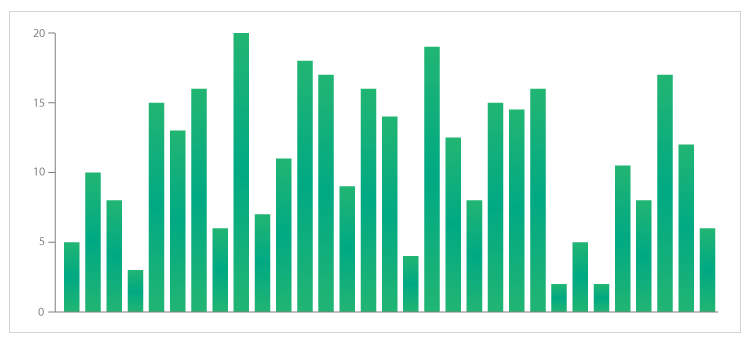
\includegraphics[width=0.4\textwidth]{figures/analysis/bar-chart} }}%
    \qquad
    \subfloat[Multi set bar chart]{{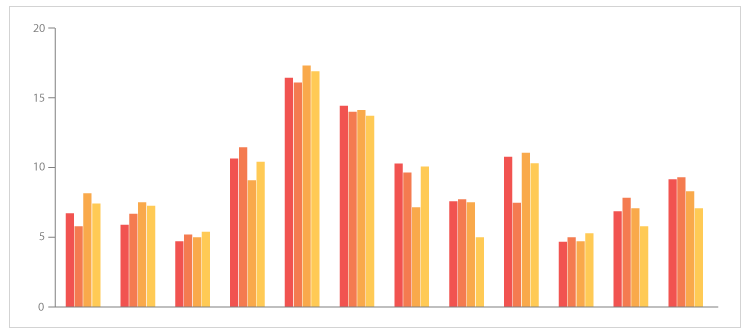
\includegraphics[width=0.4\textwidth]{figures/analysis/multiset-bar-chart} }}%
  \end{center}
  \caption{A multi set bar charts is a variation of a bar chart}
  \label{fig:analysis:bar-charts}
\end{figure}

Bar charts use either horizontal or vertical bars to show discrete, numerical comparisons across categories.
The length of a bar displays a quantitative value of a category.

Multiple bar charts display many data series next to each other.
Every series is grouped by category and a colour can be used to identify a data series.

Like line graphs, bar charts expect a \emph{tabular} data format.
In contrast to line graphs, bar charts are used to show a comparison rather than a trend.

The type of the visualization constrains the
\begin{enumerate*}[label=(\arabic*)]
    \item shape,
    \item size and, in case of a multi set bar charts,
    \item the colour
\end{enumerate*}
of the visualization.
An interaction can be shown by altering
\begin{enumerate*}[label=(\arabic*)]
    \item position,
    \item colour,
    \item shape and
    \item the texture
\end{enumerate*}
of bars and columns.
Table~\ref{tab:analysis:bar-charts:interactions} list some possible interactions.

\begin{table}
  \centering
  \caption{Interactions for bar charts}\label{tab:analysis:bar-charts:interactions}
  \begin{tabular}{ll}
    \bf Select & Highlight a bar (id of data point) \\
    \bf Encode & Change colours of data series (colours \rightarrow{} data series) \\
    \bf Reconfigure & Sort by attribute (data attribute) \\
    \bf Reconfigure & Drag bars to reorder data series (ordered list of ids of data points) \\
    \bf Filter & Hide a data series (id of data series) \\
  \end{tabular}
\end{table}

\textbf{Histograms}

\begin{figure}
  \centering
    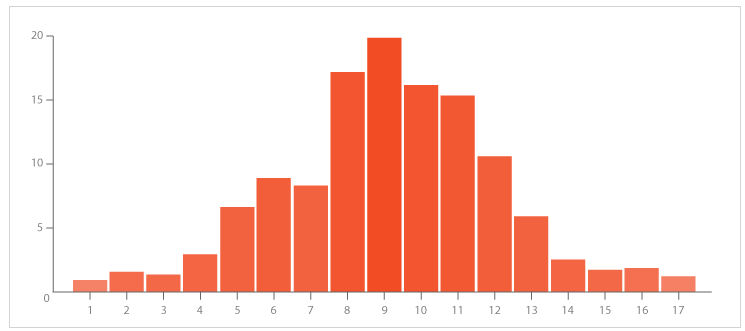
\includegraphics[width=0.4\textwidth]{figures/analysis/histogram.png}%
    \label{fig:analysis:histograms}
    \caption{A histogram is a bar chart over a continuous interval}%
\end{figure}

Histograms visualise the distribution of data over a continuous interval or certain time period.
A special type is the population pyramid, which is a pair of back-to-back histograms, one for each sex.
Histograms and bar charts expect the same kind of data, i.e.\ a \emph{tabular} format.
Almost the same interactions as in Table~\ref{tab:analysis:bar-charts:interactions} can be applied to histograms.
Except a re-ordering of bars along the x-axis, because the histogram constrains the position of bars along the interval.

\textbf{Bubble charts and scatter plots}

\begin{figure}
  \centering
    \subfloat[Bubble chart]{{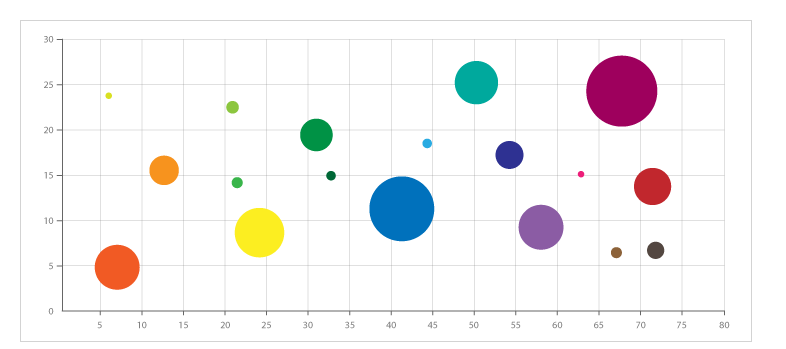
\includegraphics[width=0.4\textwidth]{figures/analysis/bubble-chart.png} }}%
    \qquad
    \subfloat[Scatter plot]{{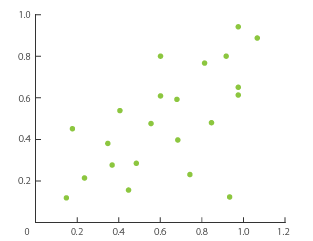
\includegraphics[width=0.4\textwidth]{figures/analysis/scatter-plot.png} }}%
    \caption{Bubble charts and scatter plots are similar regarding interactions}%
    \label{fig:analysis:bubble-chart}
\end{figure}

Both bubble charts and scatter plots are popular choices to visualize variables from two values.
Points are placed with the two values in Cartesian coordinates in order to detect relationships and correlations.
In case of bubble charts, each point is displayed as a bubble with a third value encoded in the size the bubble.
It is even possible to encode a fourth value in the colour of the bubble.

Like line graphs, bar charts and histograms, a scatter plot expects \emph{tabular} data.
Each data point can take up to four values (in case of a coloured bubble chart).
As we can see in Table~\ref{tab:analysis:bubble-charts:interactions}, interactions also include a zooming and movement of the viewpoint.
\begin{table}
  \centering
  \caption{Interactions for bubble charts}%
  \label{tab:analysis:bubble-charts:interactions}
  \begin{tabular}{ll}
    \bf Select & Highlight a bubble (id of data point) \\
    \bf Explore & Zoom in, zoom out (width and height of window) \\
    \bf Explore & Move viewpoint position (x- and y-coordinates of viewport) \\
    \bf Encode & Change mapping of colour to category (data series \rightarrow\ colour) \\
    \bf Encode & Change colour function (function value \rightarrow\ colour) \\
    \bf Encode & Change data attribute to colour (data attribute) \\
    \bf Encode & Change data attribute to size \\
    \bf Reconfigure & Sort by attribute (data attribute) \\
    \bf Reconfigure & Drag bars to reorder data series (ordered list of ids of data points) \\
    \bf Filter & Hide a data series (id of data series) \\
  \end{tabular}
\end{table}

\textbf{Stacked bar charts}

\begin{figure}
  \centering
    \subfloat[Stacked bar chart]{{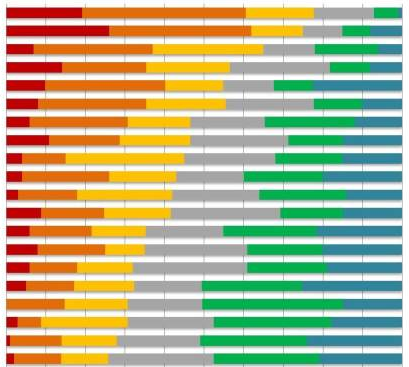
\includegraphics[width=0.3\textwidth]{figures/analysis/stacked-bar-without-baseline.png} }}%
    \qquad
    \subfloat[Stacked bar chart with baseline]{{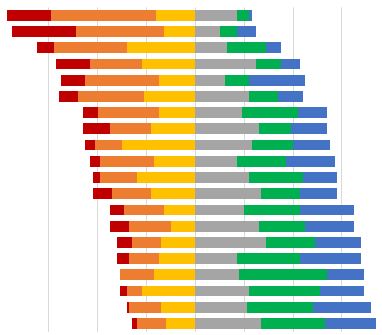
\includegraphics[width=0.3\textwidth]{figures/analysis/stacked-bar-with-baseline.png} }}%
    \caption{Stacked bar charts can be ordered along a baseline or stretch to 100\% width to show the percentage-of-the-whole of each group}%
    \label{fig:analysis:stacked-bar-chart}
\end{figure}
\begin{figure}
  \centering
    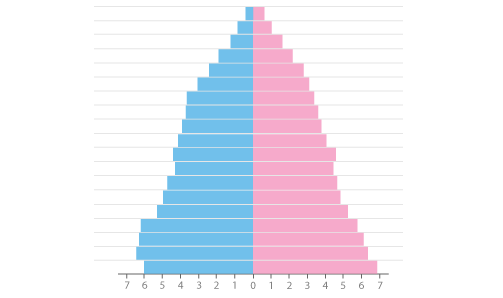
\includegraphics[width=0.4\textwidth]{figures/analysis/population-pyramid.png}%
    \label{fig:analysis:population-pyramid}
    \caption{A population pyramid can be modeled as a stacked bar chart}%
\end{figure}

Unlike a multi-set bar graph which displays their bars side-by-side, stacked bar graphs segment their bars of multiple datasets on top of each other.
A baseline, as shown in figure~\ref{fig:analysis:stacked-bar-chart} might be modeled as two back-to-back multi-set bar graphs. A reordering would e.g.\ move one data set from the left side to the right side.
A stacked bar chart also expects \emph{tabular} data
If the stacked bar chart has a baseline, often the sign of the numeric value defines the placement of the segment on the left or on the right side.
Table~\ref{tab:analysis:stacked-bar-chart:interactions} shows possible interactions, including the highlighting of a feature, a change of color mapping or a reordering of the baseline.
% \conceptTable{Tabular data, multiple date sets as series}{Size, shape, orientation.}{Color, position, texture.}

\begin{table}
  \centering
  \caption{Interactions for stacked bar charts}%
  \label{tab:analysis:stacked-bar-chart:interactions}
  \begin{tabular}{ll}
    \bf Select & Highlight a bar (id of data point) \\
    \bf Encode & Change mapping of category to colour (data series \rightarrow\ colour) \\
    \bf Reconfigure & Sort by attribute (data attribute) \\
    \bf Reconfigure & Reorder Y axis (ordered list of ids of data points) \\
    \bf Reconfigure & Sort stacking order by attribute (data attribute) \\
    \bf Reconfigure & Specify the stacking order data series (ordered list of ids of data series) \\
    \bf Reconfigure & Specify a negative data series (list of ids of data series) \\
    \bf Filter & Hide a data series (id of data series) \\
  \end{tabular}
\end{table}


\textbf{Hierarchical visualizations}

\begin{figure}
  \centering
    \subfloat[Tree map]{{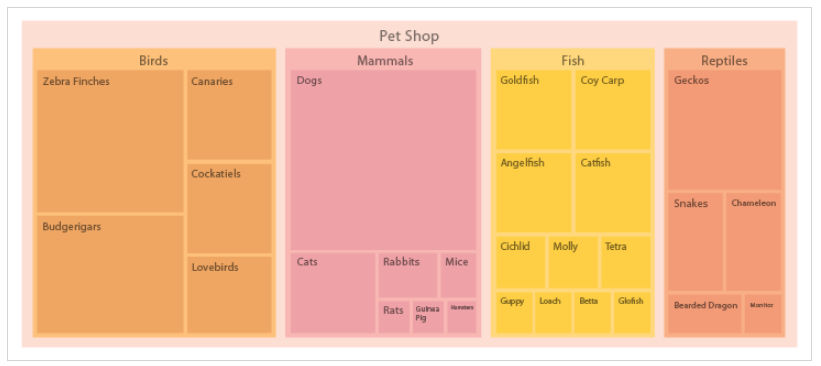
\includegraphics[width=0.4\textwidth]{figures/analysis/treemap.png} }}%
    \qquad
    \subfloat[Sunburst diagram]{{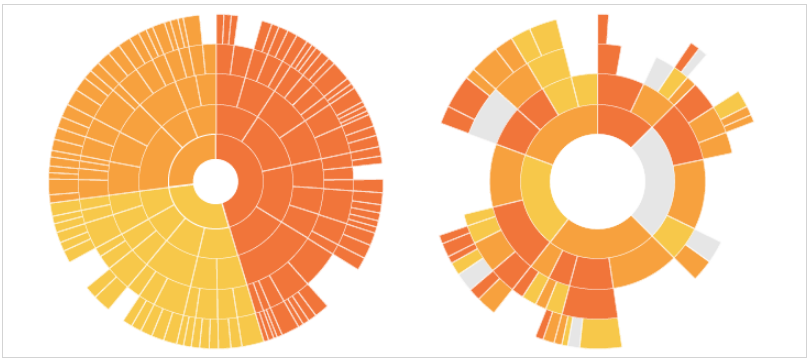
\includegraphics[width=0.4\textwidth]{figures/analysis/sunburst.png} }}%
    \caption{Tree maps and sunburst diagrams are ideal to show hierarchies}%
    \label{fig:analysis:hierarchies}
\end{figure}

Treemaps are great to show hierarchical data without ever exceeding the available screen.
Each feature is a assigned a rectangle according to a layouting algorithm.
Unlike a tree map a hierarchical ring diagram or sunburst diagram shows each level of the tree as a series of rings.

Therefore, both tree map and ring diagram expects \emph{hierarchical} data in form of a tree.
Each node needs to have at least one quantitative value for layouting, additionally, each node may be assigned a color.

As we are describing hierarchies, the maximal depth of tree may be increased or decreased.
Again, interactions could include a highlighting of features and a change of color encoding.
Both visualizations may show only a subtree.
E.g.\ a click on a box in the treemap opens another treemap focused on the subtree.
Similarly a click on a slice of the ring would surround the most external ring with the children of the feature.
Table~\ref{tab:analysis:hierarchies:interactions} gives a more comprehensive list of interactions.

% \conceptTable{Tree, each feature has a value for layouting.}{Position, Size, shape, orientation.}{Color, texture.}

\begin{table}
  \centering
  \caption{Interactions for hierarchical visualizations}%
  \label{tab:analysis:hierarchies:interactions}
  \begin{tabular}{ll}
    \bf Select & Highlight a feature (id of data point) \\
    \bf Explore & Use another node as root of the visible tree (id of data point) \\
    \bf Encode & Change mapping of category to colour (data series \rightarrow\ colour) \\
    \bf Reconfigure & Change data attribute used for layouting (data attribute) \\
    \bf Reconfigure & Sort by attribute (data attribute) \\
    \bf Reconfigure & Specify order (ordered list of ids of data points) \\
    \bf Abstract/Elaborate & Specify maximum depth of visible tree (number of levels) \\
  \end{tabular}
\end{table}

\textbf{Geographical Data}

\begin{figure}
  \centering
    \subfloat[Choropleth map]{{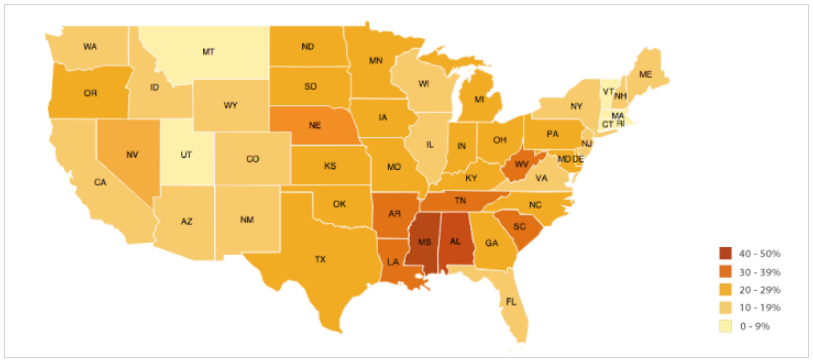
\includegraphics[width=0.4\textwidth]{figures/analysis/choropleth-map.png} }}%
    \qquad
    \subfloat[Flow map]{{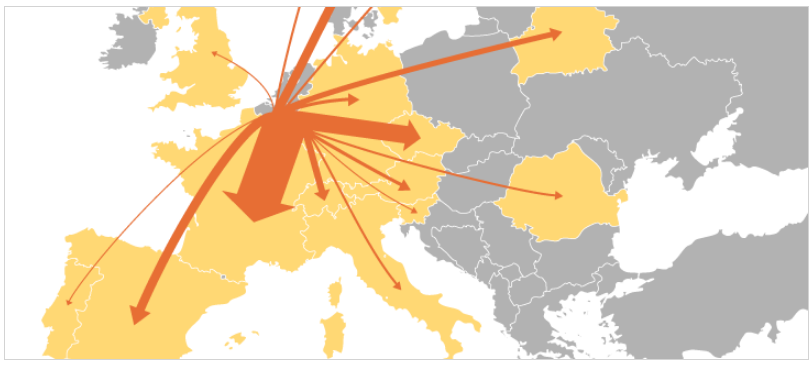
\includegraphics[width=0.4\textwidth]{figures/analysis/flow-map.png} }}%
    \caption{Choropleth maps focus on a density while flow maps show a migration of data}%
    \label{fig:analysis:geographical}
\end{figure}

Choropleth maps and flow maps are specialized diagrams focused on geographical data.
Size, position and shape of a feature is defined by the geometry data of a feature.
In choropleth maps the color of each feature is based on a data attribute.
Flow maps may display connections between features, a data value defining the size of each arrow.

Non-geographical data may be given in a \emph{tabular} form, assigned to each geographical feature.
In contrast to tabular data, a flow map expects relationships between geographical features.
Thus, it also expects \emph{relational} data in form of a graph

% \conceptTable{Graph data with edges, each feature has geometry data.}{Position, Size, shape, orientation.}{Color, texture.}

\begin{table}
  \centering
  \caption{Interactions for geographical visualizations}%
  \label{tab:analysis:geographical:interactions}
  \begin{tabular}{ll}
    \bf Select & Highlight a feature (id of data point) \\
    \bf Explore & Move viewport (latitude and longitude of viewport)\\
    \bf Explore & Zoom in, zoom out (zoom factor) \\
    \bf Encode & Change shape of marker (data id \rightarrow\ shape) \\
    \bf Encode & Change mapping of category to colour (data series \rightarrow\ colour) \\
    \bf Encode & Change colour function (value \rightarrow\ colour) \\
    \bf Encode & Change data attribute used for colour (data attribute) \\
    \bf Connect & Show relations of a feature (id of data point)  \\
    \bf Abstract/Elaborate & Change granularity of displayed regions (number of levels) \\
  \end{tabular}
\end{table}

\textbf{Activity diagrams}
\begin{figure}
  \centering
    \subfloat[Calendar]{{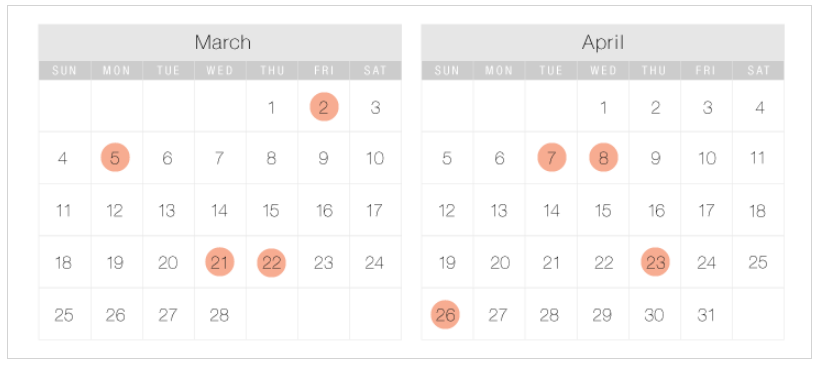
\includegraphics[width=0.4\textwidth]{figures/analysis/calendar.png} }}%
    \qquad
    \subfloat[Gantt chart]{{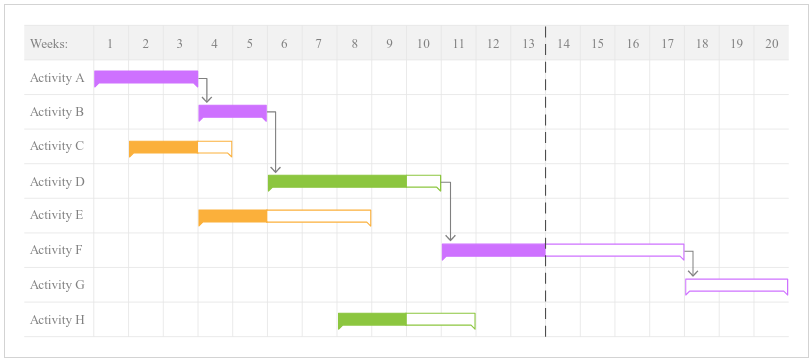
\includegraphics[width=0.4\textwidth]{figures/analysis/gantt-chart.png} }}%
    \caption{Similar to a calendar, a gantt chart shows activities and the progress along a time line}%
    \label{fig:analysis:temporal}
\end{figure}

In activity diagrams, each feature is represented as a rectangle, with the duration of the activity mapped to size and position.
Calendars and gantt charts could not only read the data from the data source, but also add new features to the data set or update metadata of a feature, e.g.\ the progress of the activity.
Calendars and gantt charts expect \emph{tabular} data, although data points might reoccur on a regular schedule.
So some data points, i.e.\ events, might repeat infinitely.

% \conceptTable{Temporal data, each feature has a time interval.}{Position, Size, orientation.}{Color, shape, texture.}

\begin{table}
  \centering
  \caption{Interactions for temporal visualizations}%
  \label{fig:analysis:temporal:interactions}
  \begin{tabular}{ll}
    \bf Select & Highlight a feature (id of data point) \\
    \bf Explore & Show a different period of dates (start and end datetime)\\
    \bf Explore & Show a different time interval (start and end hour)\\
    \bf Encode & Change color of categories or activities (data series \rightarrow\ colour) \\
    \bf Encode & Change data attribute used for colour (data attribute) \\
    \bf Filter & Remove a calendar or a category (id of data series) \\
  \end{tabular}
\end{table}

\section{Multiple View Interactions}\label{sec:analysis:examples:multiple}

\textbf{Detail view}
\begin{figure}
  \centering
  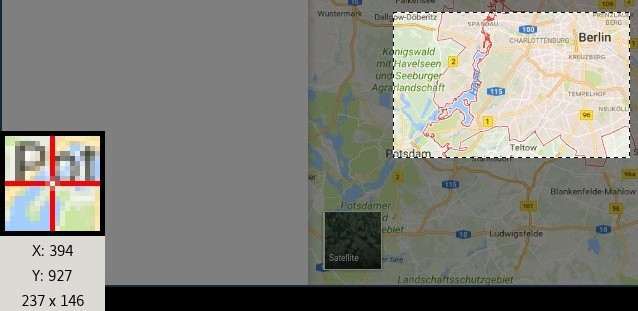
\includegraphics[width=0.4\textwidth]{figures/analysis/detail-view}
  \caption{The screenshot-tool ``shutter'' shows a magnified detail view of the area around the mouse cursor in the lower right corner of the screen}\label{fig:analysis:detail}
\end{figure}

\section{Requirements}\label{sec:analysis:requirements}
In this subsection, we list a set or requirements imposed on a \cmv{} framework.
These requirements can be used for further evaluation.
\textbf{Serialization} is the process of translating objects that can be stored or transmitted and reconstructed later.
In order to coordinate interactions among views, information needs to be passed from one view to another.
A framework for \cmvs{} should therefore find a serialization format for interactions which has
\begin{enumerate*}[label=(\arabic*)]
  \item
    small payloads and
  \item 
    fast serialization and deserialization.
\end{enumerate*}

\textbf{Reversibility} in the context of a \cmv{} framework means if it is possible to undo the effect of an interaction.
Ideally, every interaction function should have a well-defined inverse.
For every interaction that is not reversible, the computational cost to replay the interactions from the original state up to the point of the interaction should be minimal.

\textbf{Data extensibility} indicates the ease of reloading and updating data on the fly.
This is especially important if an interaction requests additional data from an external service.
We consider good extensibility when
\begin{enumerate*}[label=(\arabic*)]
  \item
    additional data attributes can be added without lookup of corresponding items and
  \item
    no de-duplication steps are necessary when new items are added.
\end{enumerate*}

\textbf{Development costs} qualify how much time and effort is needed in order to develop new components for the \cmv{} framework.
We track these costs in working days and the number of changed lines of code.


\textbf{Maintainability} means in our case, how much other views are impacted by a change of an interaction in one view and how error-prone the framework is.
In general it is hard to measure maintainability.
For the \cmv{} framework we want to measure the
\begin{enumerate*}[label=(\arabic*)]
  \item
    lines of code and the
  \item
    cycliomatic complexity. We will try to find a means to measure
  \item
    cohesion and
  \item
    coupling in the framework.
\end{enumerate*}
We assume that the amount of shared data between views is an indicator for high coupling.



\section{Comparison of client-side component frameworks}\label{sec:analysis:frontend-framework-comparison}

This section evaluates the most suitable client-side rendering and component based JavaScript framework for \cmvs{} and whether or not to use web components.

Three JavaScript frameworks have been evaluated:
\begin{enumerate*}[label=(\arabic*)]
  \item GlimmerJS
  \item Google Polymer and
  \item ReactJS.
\end{enumerate*}
Google Polymer is built on top of web components and GlimmerJS applications can be exported as a web component, but React does not support web components.

\textbf{Web components} is a recent standard of the W3C\cite{W3C2017} to bring component-based software engineering to the world wide web.
Web components are a set of web platform APIs to create new custom, reusable, encapsulated HTML tags that can be used in web pages and web applications~\cite{WebComponents2017}.
If \cmvs{} are implemented in JavaScript based web applications, web components are a promising choice, to allow arbitrary views to be put together.


\textbf{GlimmerJS} is the rendering enginge of EmberJS\cite{Ember2017}.
In 2017 it was released as a standalone component framework.
Applications written in GlimmerJS can be exported as web components.
These web components can be included in any website, which makes GlimmerJS a reasonable choice to build high-quality widgets for user interfaces.
GlimmerJS also uses handlebars\cite{Handlebars2017}, a user-friendly templating language.
The downside of GlimmerJS is the current lack of documentation and immaturity due to the recent first release this year.

\textbf{Google Polymer} is another popular library to build web components \cite{Polymer2017}.
With 18,469 stars on Github it is the most popular framework for web components at the time of writing.
Polymer has a large community and comprehensive documentation and therefore more suitable than GlimmerJS to build \cmvs{}.

But critically, \cmvs{} require a means to exchange data between views, which is specific to interactions.
The web component specification, unfortunately, does not specify how arbitrary JavaScript objects can be passed to web components.
String based attributes are supported, as seen in Listing~\ref{lst:evaluation:web-components-data}.
To pass rich data to components however, web component frameworks have to roll their own data flow and syntax.
Google Polymer's syntax to pass rich data to a components is shown in Listing~\ref{lst:evaluation:polymer-data}.
But this is a proprietary solution that abandons standard HTML.

\lstinputlisting[
  language=HTML,
  label={lst:evaluation:web-components-data},
  caption={An example of string based attributes of web components~\cite{GoogleMapWebComponent2017}}
]{listings/evaluation/web-components-data.html}

\lstinputlisting[
  language=HTML,
  label={lst:evaluation:polymer-data},
  caption={An small syntax example how Google Polymer passes rich data to a component}
]{listings/evaluation/polymer-data.html}

This raises some problems in existing applications:
A particular component-based frontend framework can not be assumed, a lot of existing applications are also written without any JavaScript framework.
Proprietary solutions like the one of Polymer lessen the main motivation of implementing against web components:
Platform agnostic flexibility.

\textbf{ReactJS} is a JavaScript library for building user interfaces\cite{React2017}.
React is explicitly not implementing web components and is not going to implement web components in the future.
It has, in return, a well-known way of integrating the component framework into a legacy application built with e.g.\ jQuery.
Along with its major advantage of easy integration, it has a striving community, lots of documentation and tutorials and it is well tested.

As a summary, if there is
\begin{enumerate*}[label=(\arabic*)]
  \item no obligation to implement web components
  \item and an easy integration into an existing application is necessary,
\end{enumerate*}
then React is the perfect choice for \cmvs{}.
Figure~\ref{fig:implementation:frontend-frameworks} shows the pros and cons of each framework for the use case.

\begin{figure}[h]
  \centering
  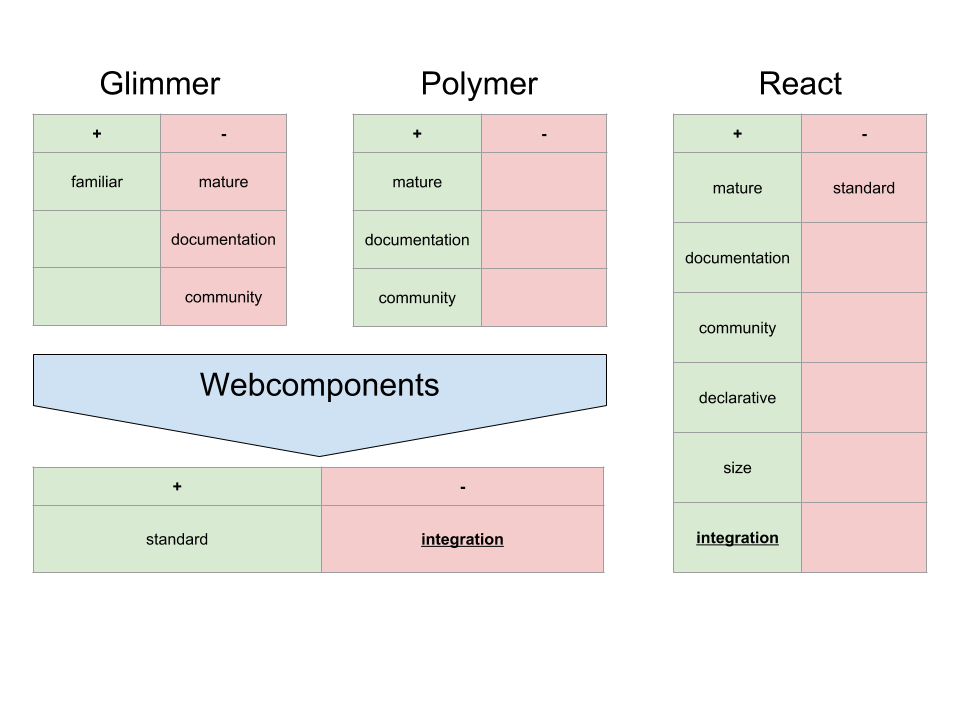
\includegraphics[width=\textwidth]{images/frontend-frameworks.png}
  \caption{Comparison of frontend frameworks}\label{fig:implementation:frontend-frameworks}
\end{figure}

